\documentclass[conference]{IEEEtran}
\IEEEoverridecommandlockouts
% The preceding line is only needed to identify funding in the first footnote. If that is unneeded, please comment it out.
\usepackage{cite}
\usepackage{amsmath,amssymb,amsfonts}
\usepackage{algorithmic}
\usepackage{graphicx}
\usepackage{textcomp}
\usepackage{xcolor}
\usepackage{svg}
\usepackage[backgroundcolor=red!50]{todonotes}
\def\BibTeX{{\rm B\kern-.05em{\sc i\kern-.025em b}\kern-.08em
    T\kern-.1667em\lower.7ex\hbox{E}\kern-.125emX}}

%% To do notes set up
\setuptodonotes{inline}
\begin{document}

\title{A memristor based stochastic number generator for low cost arithmatic \\
{\footnotesize \textsuperscript{}with image processing case study}
}

\author{\IEEEauthorblockN{Tanner Robison}
\IEEEauthorblockA{\textit{Electrical and Computer Engineering} \\
\textit{Portland State University}\\
Portland, Oregon \\
tnr@pdx.edu}
\and
\IEEEauthorblockN{Ivan Flores Suares}
\IEEEauthorblockA{\textit{Electrical and Computer Engineering} \\
\textit{Portland State University}\\
Portland, Oregon \\
ivanf@pdx.edu}
\and
\IEEEauthorblockN{Ren Cadua}
\IEEEauthorblockA{\textit{Electrical and Computer Engineering} \\
\textit{Portland State University}\\
Portland, Oregon \\
rencadua@pdx.edu}
}

\maketitle

\begin{abstract}
    Edge computing devices face substantial area, power, and reliability constraints,
    though most of their workloads like image processing or neural network inferancing
    tolerate small computational errors, making them suitable for stochastic 
    computing (SC). SC encodes values as the probability of a 1 appearing in a random
    bit stream. aritmatic with this is simplified to single gates, with multiplication
    being done with an and gate, and scaled addition with a
    multiplexer. individual bit errors have only a minor effect on the result.
    The stochastic number generators (SNGs) that produce the random bitstreams usually
    dominate the cost of these systems, reducing the validity of the advantages. 
    This paper proposes using a behavioral SNG model using the memristor stochastic
    switching model proposed by Naous et al with which
    pseudorandom values are compared with the voltage dependent switching probability.
    This presents the applied voltage as a control knob for setting the stochastic value.
    We will pair the SNG with a multiplier and scaled adder and evaluate the circuit
    in 2 ways. The encoding accuracy for the voltage to probability mapping. 
    The arithmatic error as a function of bitstream length.
    An additional stretch goal of the project will be to implement the unit into
    an image processing case study to reveal the effects of progressive precision
    and graceful degredation.

\end{abstract}

\begin{IEEEkeywords}
stochastic, memristors, arithmatic, image processing, SystemVerilog, FPGA
\end{IEEEkeywords}

\section{Introduction}
Current edge computing devices like IoT, wearables, or biomedical implants rely
more and more on local processing for stronger real time capabilities, But face
limited area, power, and reliability constraints. Many of the workloads these devices work
with are error tolerant like image processing, neural network inferancing, or 
signal filtering meaning they accept small numerical errors without changing the result.
conventional binary arithmatic wastes area and power computing exact results that 
these workloads dont need while facing larger consequences to incorrect bit errors.
Stochastic computing presents as a useful computing paradigm for these types of workloads
by way of simplified arithmatic gate construction. Arithmatic like multiplication, and
addition can be done with singular gates. The circuitry needed to generate stochastic
streams is the current hangup with the paradigm, and usually dominates the cost of these
systems offsetting the advantages of the simpler arithmatic.

Memristors are non-volatile devices whose resistances depend on an internal state variable.
The changing of this resistance is know as the switching characteristic and is
inherintly probabilistic. Naous et al \cite{memristor_stochasticity} modeled this
behavior as a voltage dependent switching probability. This maps a voltage to a 
probability, which presents the voltage as a natural control knob for setting a 
stochastic value.

This paper proposes using this voltage dependent switching probability to create a
behavioral Stochastic Number Generator (SNG) model implemented on an FPGA. 
The model will work by comparing pseudorandom
values with the $P_{switch}(V)$ equation allowing for the applied voltage control knob.
The SNG will be paired with a scaled adder and multiplier to perform arithmatic on
these streams and the device will be evaluated in 2 ways: The encoding accuracy for the
voltage to probability mapping, and the arithmatic error as a function of the bit
stream length.

\section{Background}
\subsection{Stochastic Computing}
stochastic computing (SC) is a hardware level paradigm of probabilistic computing.
Numerical values are encoded with the probability of a 1 appearing in a random bitstream
\cite{stochastic_computing},
and the bits position in the stream does not matter. This is what makes SC suitable
for error tolerant workloads, a wrong bit in binary has exponential consequences as the
bit works up to the most significant bit position. Because a bits position in the
stream does not matter this consequence does not exist.
This allows for complex arithmatic 
to be executed with simpler logic gates over conventional binary operations. 
For example, to multiply two stochastic bit streams together is just one gate, 
for unipolar numbers[0,1] this an \textbf{and} gate, and 
for bipolar numbers[-1,1] this is an \textbf{XNOR} gate \cite{stochastic_computing_systems}. 
To do the same operation in positional binary would require many gates.
Addition is done with a 2:1 multiplexer, and requires a 3rd stochastic stream. The
select for the MUX must be supplied with the new stream strictly with a value of 0.5
\cite{stochastic_computing_systems}. Given input streams A and B the output is 1 
with probability \cite{stochastic_computing_systems}
\begin{equation}
    0.5\,p_A + 0.5\,p_B = (p_A + p_B)/2
\end{equation}

The result is scaled by $1/2$ because a probability can't exceed 1, so the sum of
2 values must be mapped back into that range. The MUX circuit can perform scaled addition
for both unipolor and bipolar numbers. This requires multiplying $2 * Number of addition operations$
after converting back to binary to get the true value.

To convert back to binary requires a counter that counts the number of 1's over L cycles.
where L is the bit stream length.
The Trade off comes with time, because to get N bits of precision from
a bitstream requires $2^N$ clock cycles or more once you account for things like correlation
and noise. This results in latency growing exponentially as precision grows, where
8 bit precision requires 256 cycles, but 16 bit requires 65,536. Low gate count
does not necessarily mean low energy per result, because energy is the product of
power and computation time, energy per result also scales exponentially with time.
With these considerations Stochastic computing is mainly suited for highly parallel,
error tolerant, and low precision workloads. \cite{manohar2015}
Some example applications where this is useful are in neural network accelerators\cite{nna},
FIR filters\cite{firfilters}, biomedical signal processing\cite{biomedical}, 
image processing\cite{imageprocessing}, audio filtering\cite{audiofiltering}, etc....

\subsection{Correlation}

In statistics, correlation is the tendency of two random variables to move
together, so that knowing the value of one provides some information about the
other. In stochastic computing, correlation describes how the positions of
the 1s in two bitstreams line up, independent of how many 1s each stream
contains. This matters because the function a gate computes depends on that
alignment: multiplication and scaled addition are only computed correctly when
their input streams, including the MUX select stream, are statistically independent \cite{sn_stream_independance}. For example, one might try to
square a stream encoding 0.5 by feeding it into both inputs of an AND gate,
but the result is 0.5 rather than 0.25, because each bit is simply ANDed with
itself \cite{survey_of_stochastic_computing}. Delaying one copy does not
necessarily solve the problem: delaying the stream 01010101 by one cycle
produces 10101010, and the AND gate now outputs 0. This failure is caused by
\emph{autocorrelation}, the correlation between a stream and a time-shifted
copy of itself, which is high for periodic streams.

Ordinary correlation is poorly suited to bitstreams, because its
achievable range depends on the values the streams encode. Alaghi and Hayes
introduced the stochastic computing correlation (SCC) measure
\cite{sn_stream_independance}, which compares the observed overlap of 1s, $P(A \wedge B)$, with
the overlap expected for independent streams, $p_A p_B$, normalized by the
maximum or minimum overlap possible:
\begin{equation}
\mathrm{SCC} =
\begin{cases}
\dfrac{P(A \wedge B) - p_A p_B}{\min(p_A, p_B) - p_A p_B}, & P(A \wedge B) > p_A p_B \\[2ex]
\dfrac{P(A \wedge B) - p_A p_B}{p_A p_B - \max(p_A + p_B - 1,\, 0)}, & \text{otherwise}
\end{cases}
\end{equation}
An SCC of 0 indicates independent streams, $+1$ indicates the maximum possible
overlap, and $-1$ the minimum. Correlation is not always harmful: with
$\mathrm{SCC} = +1$, an AND gate computes $\min(p_A, p_B)$ and an XOR gate
computes $|p_A - p_B|$ \cite{sn_stream_independance}. In practice, independent streams are
produced by driving each SNG with its own LFSR. Because LFSRs that share a
feedback polynomial produce time-shifted copies of the same sequence, accuracy
improves when each LFSR uses a different feedback polynomial as well as a
different seed \cite{LFSR_seeding}.

\subsection{Stochastic Number Generators}
A stochastic number generator (SNG) converts an $n$-bit binary value $X$ into
a stochastic bitstream. The conventional design pairs a random number source
with an $n$-bit binary comparator. Each clock cycle, an $n$-bit random number
$R$ is compared with $X$, and the SNG outputs a 1 if $R < X$ and a 0
otherwise, so each output bit is 1 with probability $X/2^n$. The random
source is typically a maximal-length $n$-bit linear feedback shift register
(LFSR), which cycles pseudo-randomly through $2^n - 1$ states using only $n$
flip-flops and a few XOR gates. Because the accuracy of stochastic arithmetic
depends on the quality of these streams, the LFSR's seed and feedback
polynomial measurably affect computational accuracy \cite{LFSR_seeding}.
Low-discrepancy sequences can replace the LFSR to make streams converge
faster, at the cost of additional hardware \cite{low_discrepancy}.

Although the arithmetic in a stochastic system may be a single gate, every
independent input stream requires its own SNG, consisting of an $n$-bit
register, feedback logic, and an $n$-bit comparator. As a result, SNGs rather
than the arithmetic logic usually dominate the cost of stochastic systems:
CMOS-based SNGs have been reported to consume over 80\% of a stochastic
system's power and area \cite{sng_cost_reram}, and up to 80\% of total design
area \cite{scrimp}. Sharing one random source among several SNGs reduces this
cost, but it introduces correlation between the resulting streams, which
breaks operations such as multiplication that require independent inputs.
This trade-off between SNG cost and stream independence motivates the search
for SNGs built from emerging devices with intrinsic randomness, such as
memristors.

\subsection{Memristors}

A memristive device is a circuit element who's electrical behavior depends on an 
internal state that is influenced by its previous electrical excitation. The 
memristor was originally proposed in theory by Chua in 1971 \cite{chua1971memristor}
as a relationship between charge and magnetic flux. It was later generalized to 
memristive systems where the device resistance can depend on one or more internal 
state variables with the strukov et al paper \cite{Strukov2008}.

A voltage controlled memristive system can generally be represented as
\begin{equation}
    i(t) = G(x,v,t)v(t)
\end{equation}

\begin{equation}
    \frac{dx}{dt} = f(x,v,t)
\end{equation}

where x represents the internal device state, G is the state dependant conductance, 
and f describes how the state changes in response to an applied voltage. 
The state dependance distinguishes the system from an ordinary resistor where
\begin{equation}
    i(t)=\frac{v(t)}{R}
\end{equation}

In a memristor an applied voltage can alter the device state, changing the conductance. 
This can be good because it means we can program the resistance at any time, 
but also means the electrical operation (voltage pulse) used to evaluate a 
computational result can disturb the value stored by the device.

Memristor switching is also random. Apply the same voltage pulse many times,
and the device will switch on some tries but not others. How often it
switches depends on the pulse voltage magnitude, with higher voltages switching more
often~\cite{memristor_stochasticity}. This randomness is a problem for
memory, but it is exactly what stochastic computing needs: pulsing a
memristor once per clock cycle produces a random bitstream whose fraction of
1s is set by the voltage~\cite{gaba2013stochastic}.

\section{Proposed Design \& Methodology}

\subsection{FPGA Design}
The system will be implemented in SystemVerilog and deployed on a Basys~3
(Artix-7) FPGA using Vivado, clocked by the board's 100~MHz oscillator.
Fig.~\ref{fig:block} shows the datapath. Because the FPGA contains no
memristive devices, the SNG is a behavioral emulation: it reproduces the
voltage-to-probability encoding of the stochastic switching model of Naous
et al.~\cite{memristor_stochasticity}, while a pseudorandom source supplies
the randomness that a physical device would provide intrinsically.

The probability that a write pulse of amplitude $V$ and width $\Delta t$
switches the memristor is
\begin{equation}
  P_{switch}(V) = 1 - e^{-\Delta t/\tau(V)}, \qquad
  \tau(V) = \tau_0\, e^{-V/V_0},
  \label{eq:pswitch}
\end{equation}
with variables defined in the Appendix. We use the fitted values
$\tau_0 \approx 2.69\times10^{5}$~s and $V_0 \approx 0.163$~V
from~\cite{memristor_stochasticity} and a pulse width of $\Delta t = 1$~ms.
Each clock cycle emulates one write pulse followed by an ideal reset, so
successive output bits are independent.

Each SNG pairs a 16-bit LFSR with its own lookup table (LUT) and a
comparator. Every LUT has 2048 entries, one per voltage code, and entry $k$
stores the 16-bit threshold
$T_k = \mathrm{round}\big(P_{switch}(V_k)\,(2^{16}-1)\big)$. At the start of
a run, the SNG's voltage code selects its threshold, and each cycle the SNG
outputs a 1 when the LFSR value is less than or equal to that threshold, so
the fraction of 1s in the stream approximates $P_{switch}(V_k)$. Each LUT is
generated from slightly perturbed device parameters, emulating
device-to-device variation. The LUTs are generated by a Python script and loaded 
into block RAM at synthesis using \texttt{\$readmemh}; all three together occupy 
96~Kbit of the Basys~3's 1.8~Mbit of block RAM.

With $\Delta t = 1$~ms and a margin for device variation, the 2048 codes span
approximately 1.4~V to 4.0~V, a resolution of about 1.28~mV per code. This
range extends beyond the 2.6--3.6~V measurements used to fit the model, so
switching probabilities near either end of the range are
extrapolated~\cite{memristor_stochasticity}.

The design contains three SNGs. Two produce the operand streams $a$ and $b$,
and the third produces the adder's select stream $s$, using the entry of its
own LUT closest to 0.5. Each LFSR uses a distinct feedback polynomial and
seed so that the three streams are independent, and its period of 65,535 cycles is longer than the longest
bitstream. Multiplication is a single AND gate and scaled addition a 2:1
multiplexer, both implemented directly in FPGA logic.

Counters accumulate the 1s on each SNG stream and on both arithmetic outputs
over $L$ cycles, with $L$ ranging from $2^{4}$ to $2^{15}$, and return the
counts over UART to a Python host script. The host computes each SNG's
encoding accuracy by comparing its measured fraction of 1s with
$P_{switch}(V_k)$, and the arithmetic error by comparing the AND and MUX
outputs with the exact product and scaled sum. 
Operand codes are chosen from each device's own LUT, so the measured error 
reflects the stochastic computation rather than device variation.

A control finite-state machine (FSM) coordinates each run in five states.
In IDLE, it waits for a start byte from the host. In RECEIVE, it collects a
fixed 14-byte packet containing the three voltage codes, three LFSR seeds,
and the bitstream length $L$, and stores them in configuration registers;
a timeout returns it to IDLE if the packet is incomplete. In LOAD, each SNG
reads its threshold from its LUT, the LFSRs are loaded with their seeds,
and the counters are cleared. In RUN, the SNGs, arithmetic gates, and
counters operate for $L$ clock cycles. In REPORT, the five 16-bit counts
are returned to the host as 10 bytes, and the FSM returns to IDLE. A run
takes about 2.5~ms, dominated by UART transfer time, so sweeping all 2048
voltage codes at one bitstream length takes about 5~s.

\begin{figure}[h]
  \centering
  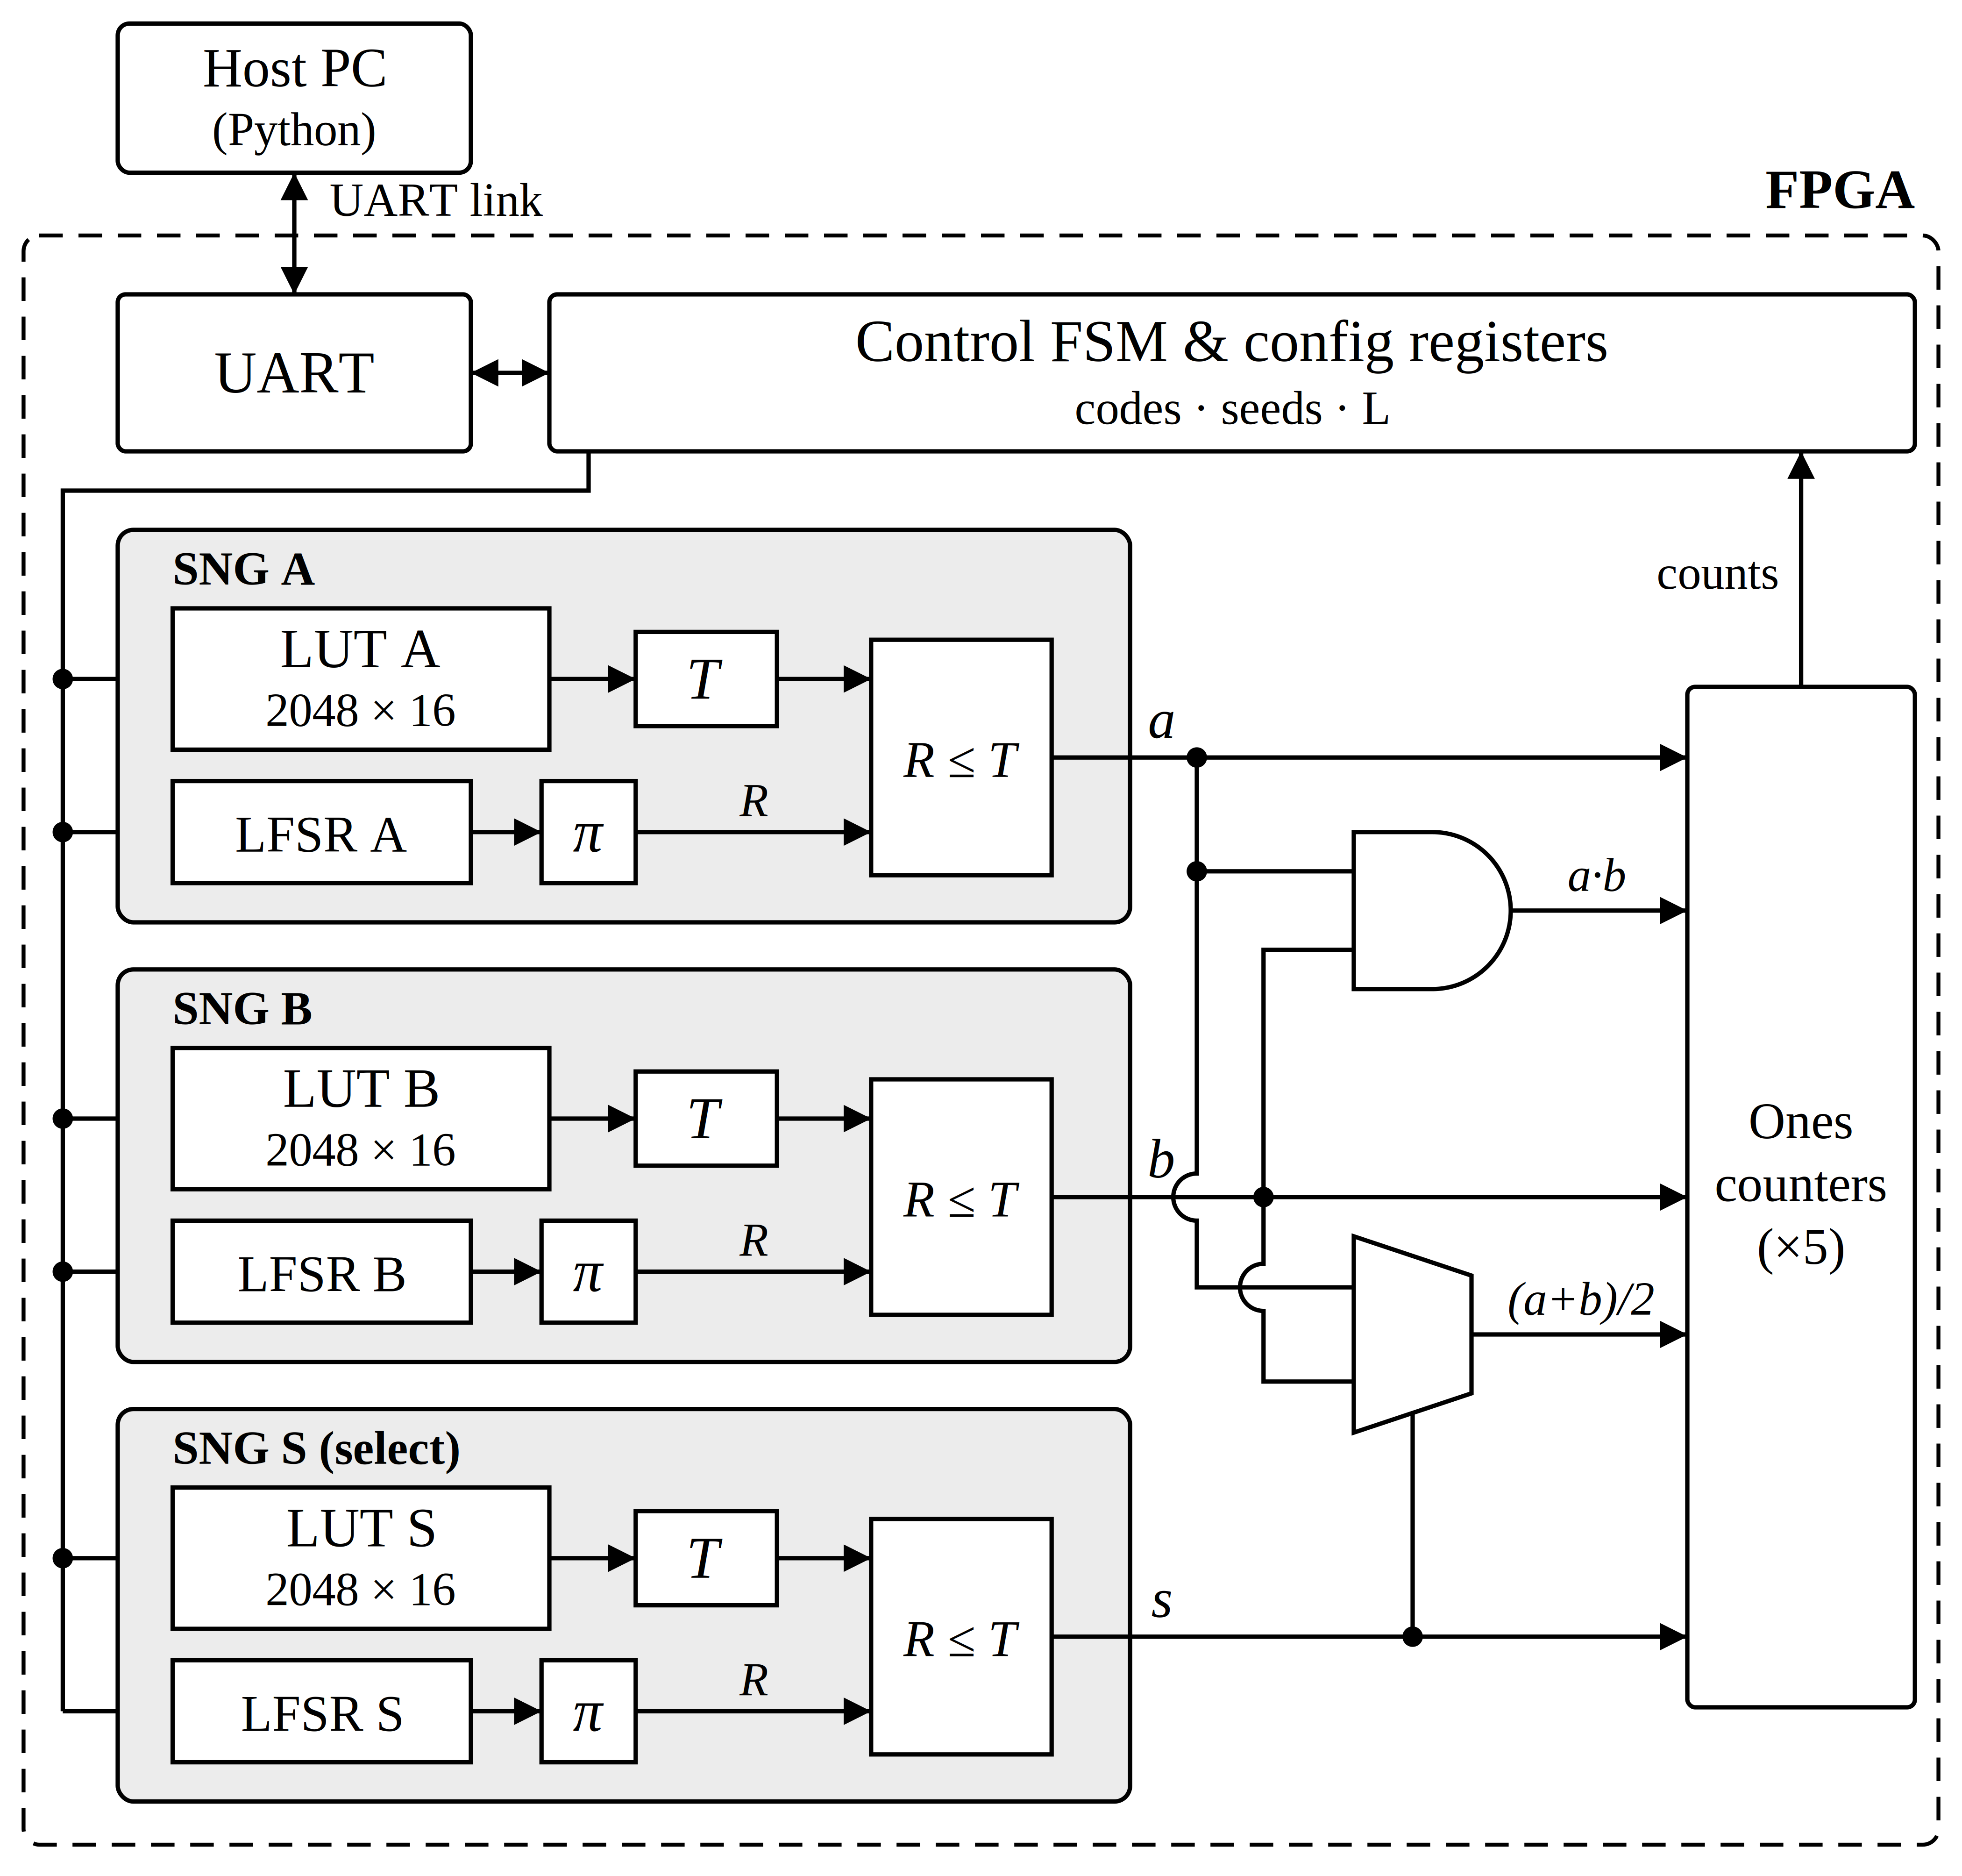
\includegraphics[width=\columnwidth]{block_diagram.png}
  \caption{Datapath. Each SNG's voltage code indexes that SNG's own
    $P_{switch}$ LUT, generated from perturbed device parameters. 
    The returned thresholds are latched and compared with
    independent LFSRs to produce stochastic streams, which drive the AND
    multiplier and MUX adder. Ones are counted over $L$ cycles and reported
    to the host over UART.}
  \label{fig:block}
\end{figure}

\begin{figure}[h]
    \centering
    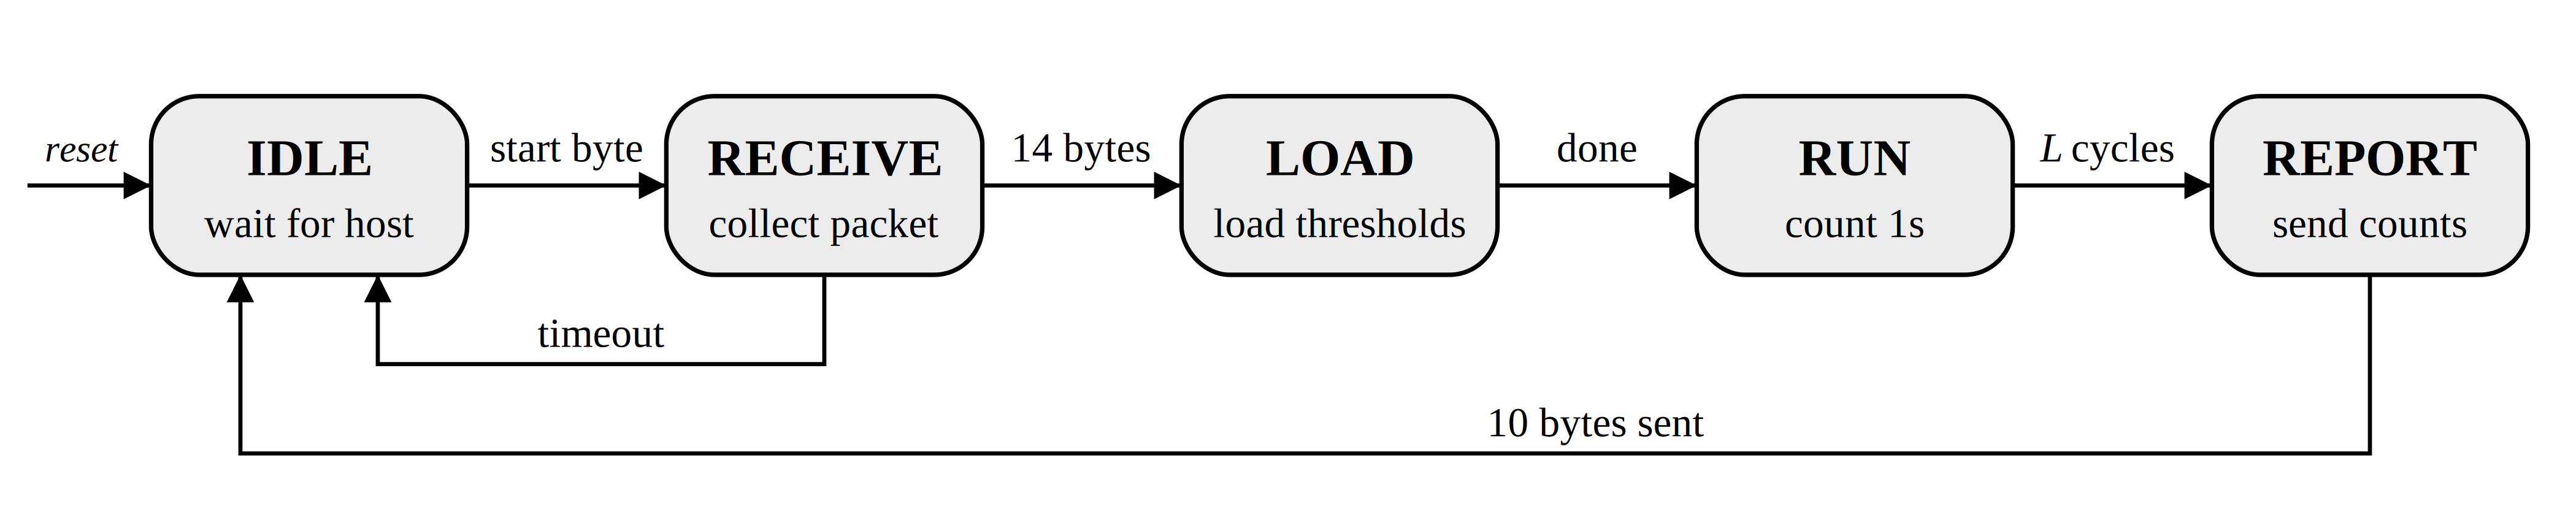
\includegraphics[width=\columnwidth]{fsm_diagram.png}
    \caption{Block diagram of the FSM controller, Each run receives a 14-byte configuration packet,
    loads thresholds and seeds, runs the SNGs for $L$ cycles, and returns
    the five counts. An incomplete packet times out back to IDLE.}
    \label{fig:fsm}
\end{figure}

\subsection{Image Processing Case Study}
As a stretch goal, the arithmetic unit will be applied to grayscale images.
Rather than storing images on the FPGA, the host will stream them over the
same UART link one pixel at a time: it converts each 8-bit intensity to a
voltage code, the FPGA runs the stochastic operation for $L$ cycles, and the
returned count becomes the output pixel. Scaled addition blends two images,
and multiplication applies a mask or brightness scale. At 115,200~baud, a
$128\times128$ image takes on the order of ten seconds per pass, which is
acceptable for an offline study. Repeating each operation at increasing $L$
demonstrates progressive precision, with output quality measured by Peak Signal
to Noise Ratio (PSNR)
against a floating-point reference.

\newpage
\section{Timeline}
\begin{itemize}
  \item \textbf{Week 1:} Python switching model, LUT generation, start on  LFSR 
      and SNG RTL.
  \item \textbf{Week 2:} complete week 1 work, control FSM, and UART RTL;
        verify in simulation against the Python model.
  \item \textbf{Week 3:} Synthesize for the Basys~3; complete host script
        and test it against a Python emulation of the FPGA. Begin board
        bring-up if hardware delivered
  \item \textbf{Week 4:} Board bring-up, confirm hardware counts match
        simulation run encoding-accuracy and arithmetic-error sweeps.
  \item \textbf{Week 5:} Analysis and figures image case study if on
        schedule.
  \item \textbf{Week 6:} Final report.
\end{itemize}

\section{Conclusion}
Stochastic computing reduces arithmetic to single logic gates, but the
stochastic number generators (SNGs) that feed those gates dominate the cost
of stochastic systems. This project proposes an SNG built on the
voltage-dependent switching probability of memristors, using the stochastic
switching model of Naous et al.~\cite{memristor_stochasticity} so that the
applied voltage directly sets the value a bitstream encodes. The SNG will be
emulated in SystemVerilog on a Basys~3 FPGA, with a separate lookup table
for each device to model device-to-device variation and an LFSR standing in
for the device's intrinsic randomness. Three such SNGs will drive an
AND-gate multiplier and a MUX-based scaled adder, and a control FSM will run
each experiment and report results to a host computer over UART.

The design will be evaluated on two measures: how accurately each SNG
reproduces its device's switching probability, and the error of the
multiplier and adder as a function of bitstream length. We expect both
errors to fall roughly as $1/\sqrt{L}$, halving with each fourfold increase
in bitstream length. Because the FPGA emulates memristors rather than
containing them, this work does not measure hardware savings; instead, it
tests whether voltage-controlled switching probability can serve as an
accurate encoding for stochastic arithmetic, a prerequisite for building
such SNGs from physical devices. If time permits, an image processing case
study will demonstrate progressive precision, with output quality improving
as bitstream length increases.

\section*{Acknowledgment}
"The authors declare that generative AI was used for proofreading and editing 
assistance in the preparation of this manuscript. Figures 1 and  2 uses an AI generated
illlustration. some AI-generated content was included in the proposed design \& Methodology
section to aid in more detailed project planning and content comprehension.

\appendix
\textbf{witching Model Variables}
 
Equation 6 \& 7:
\[
  P_{switch}(V) = 1 - e^{-\Delta t/\tau(V)}, \qquad \tau(V) = \tau_0\, e^{-V/V_0}
\]
 
\noindent
$P_{switch}$ -- Probability that one voltage pulse switches the memristor.\\
$V$ -- Applied pulse voltage.\\
$\Delta t$ -- Pulse width.\\
$\tau(V)$ -- Characteristic switching time at voltage $V$.\\
$\tau_0$ -- Characteristic switching time at 0~V.\\
$V_0$ -- Voltage increase that shortens $\tau$ by a factor of $e$.\\
$e$ -- Euler's number, 2.718.

\textbf{Peak Signal-to-Noise Ratio}

PSNR measures how close an output image is to a reference image. Higher
values mean a closer match.
\[
  \mathrm{PSNR} = 10\log_{10}\!\left(\frac{MAX^2}{MSE}\right), \qquad
\]

\[
  MSE = \frac{1}{MN}\sum_{i=1}^{M}\sum_{j=1}^{N}\big(I(i,j) - K(i,j)\big)^2
\]

\noindent
$\mathrm{PSNR}$ -- Peak signal-to-noise ratio, in decibels (dB).\\
$MAX$ -- Largest possible pixel value, 255 for 8-bit grayscale.\\
$MSE$ -- Mean squared error between the two images.\\
$M, N$ -- Image height and width in pixels.\\
$I(i,j)$ -- Reference pixel value, computed exactly in floating point.\\
$K(i,j)$ -- Pixel value produced by the stochastic hardware.

\bibliographystyle{plain}
\bibliography{citations}
\end{document}
